\section{Propriedade da Equipartição Assintótica}

\begin{frame}%[allowframebreaks]
  \frametitle{Propriedade da Equipartição Assintótica}
  \begin{itemize}
  \item Vamos considerar blocos de realizações de uma variável aleatória 
        (i.e., vetores aleatórios de comprimento $n$). $n = \text{tamanho do bloco}$.
  \item Sejam $X_1, X_2, \ldots, X_n$ v.a.s i.i.d. com distribuição $p$ (dizemos
        $X_i \sim p(x)$).
  \item Existem $K$ símbolos possíveis (alfabeto ou espaço-estado de tamanho $K$), então
        $X_i \in \{a_1, a_2, \ldots, a_K\}$.
  \item Consideram $n$ variáveis aleatórias $(X_1, X_2, \ldots, X_n)$, existem $K^n$ possíveis
        realizações.
  \end{itemize}
\end{frame}


\begin{frame}%[allowframebreaks]
  \frametitle{Propriedade da Equipartição Assintótica}
  Suponha que desejamos codificar as $K^n$ possíveis realizações com uma sequência de
  dígitos binários de comprimento $m$. Então, existem $2^m$ palavras de código (\textit{codewords}).
  
  \begin{figure}[h!]
  \centering
  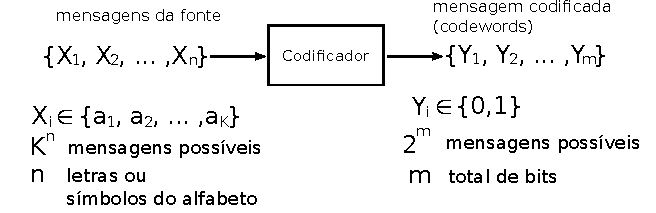
\includegraphics[width=0.7\textwidth]{images/blockcoding.pdf}
  %\caption{.}
  \label{fig:blockcoding}
  \end{figure}
 
  \begin{itemize}
  \item Para que seja possível termos uma palavra de código para cada mensagem possível,
  devemos satisfazer a seguinte condição:
        \begin{equation}
        2^m \geq K^n
        \end{equation}
        ou seja
        \begin{equation}
        m \geq (\log K) n
        \end{equation}
  \end{itemize}
\end{frame}


\begin{frame}%[allowframebreaks]
  \frametitle{Propriedade da Equipartição Assintótica}
  \begin{itemize}
  \item Quantos bits por letra da fonte utilizamos?
        \begin{equation}
        \text{taxa} = \frac{m}{n} \geq \log K \text{ bits por letra da fonte}
        \end{equation}
        Exemplo: 26 letras, precisaremos de $\lceil \log K \rceil = 5 \text{bits}$.
  \item Podemos utilizar menos bits por símbolo emitido pela fonte (na média) e ainda sim
        não ter erro? Sim.
  \item Algumas mensagens da fonte poderiam não ter a elas um código associado.

  \begin{figure}[h!]
  \centering
  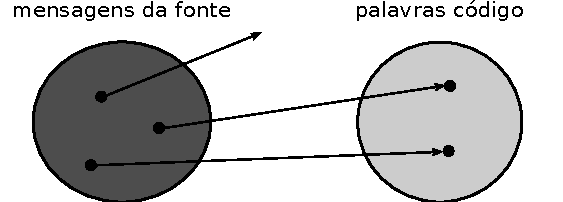
\includegraphics[width=0.5\textwidth]{images/cword-map.pdf}
  %\caption{.}
  \label{fig:cword-map}
  \end{figure}

  \end{itemize}
\end{frame}


\begin{frame}%[allowframebreaks]
  \frametitle{Propriedade da Equipartição Assintótica}
  \begin{itemize}
  \item Ao invés de descartar algumas mensagens, podemos associar a elas palavras longas
        e às outras palavras associamos palavras curtas.

  \begin{figure}[h!]
  \centering   
  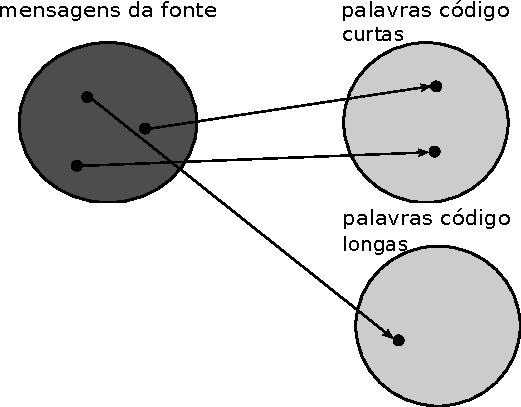
\includegraphics[width=0.35\textwidth]{images/cword-map2.pdf}
  %\caption{.}
  \label{fig:cword-map}
  \end{figure}

  \item Em qualquer um dos casos, quando $n$ é grande suficiente, podemos fazer com que a
        probabilidade, de se obter uma dessas mensagens da fonte que gerariam erro 
        (ou que teriam palavras longas associadas), muito pequena.

  \end{itemize}
\end{frame}


\begin{frame}%[allowframebreaks]
  \frametitle{Probabilidade de Palavras da Fonte}
  \begin{itemize}
  \item A probabilidade de palavras da fonte i.i.d. pode ser expressa por
        \begin{equation}
        p(X_1 = x_1, X_2 = x_2, \ldots, X_n = x_n) = \prod_{i=1}^{n} p(X_i = x_i)
        \end{equation}
  \item A informação (Shannon/Hartley) sobre um evento é dada por $-\log p(x) = I(x)$, então
        \begin{eqnarray}
        I(x_1,x_2,\ldots,x_n) &=& - \log p(x_1, x_2, \ldots, x_n) = - \log \prod_{i=1}^n p(x_i) \nonumber \\
                        &=& \sum_{i=1}^n - \log p(x_i) = \sum_{i=1}^n I(x_i)
        \end{eqnarray}
  \item Eventos independentes são aditivos em relação a esta função de informação.
  \item Note que: $E I(X) = H(X)$.
  \item A lei fraca dos grandes números diz que $\frac{1}{n} S_n \xrightarrow{p} \mu$, onde $S_n$ é a soma
        de v.a.s i.i.d. com média $\mu = E X_i$.
  \item $I(X_i)$ também é uma v.a. com média $H(X)$.
  \end{itemize}
\end{frame}
\note{
\textbf{Lei dos Grandes Números}

Se um evento de probabilidade $p$ é observado repetidamente em ocasiões independentes, 
a proporção da frequência observada deste evento em relação ao total número de repetições 
converge em direção a $p$ à medida que o número de repetições se torna arbitrariamente grande.

\vspace{1cm}

Sejam $X_1, X_2, \ldots, X_n$ v.a.s i.i.d. com $\E X_i = \mu$ e $\Var X_i = \sigma^2 < \infty$, para $i=1,\ldots,n$.
Seja a média definida por $\overline{X_n} = \frac{1}{n} \sum_{i=1}^{n} X_i$, então, para $\varepsilon > 0$,
a \textbf{Lei Fraca dos Grandes Números} diz que $\overline{X_n}$ converge em probabilidade para $\mu$, ou seja,
\begin{equation}
\lim_{n \rightarrow \infty} P \left( \vert \overline{X_n} - \mu \vert < \varepsilon  \right) = 1 .
\end{equation}
}

\begin{frame}%[allowframebreaks]
  \frametitle{Lei fraca dos grandes números e Entropia}
  \begin{itemize}
  \item Combinando o que vimos anteriormente, obtemos
        \begin{equation}
        \frac{1}{n} \sum_{i=1}^n I(X_i) \xrightarrow[n \rightarrow \infty]{p} H(X)
        \end{equation}
  \item Se $n$ fica grande suficiente, obteremos
        \begin{eqnarray}
        \frac{1}{n} \sum_{i=1}^n I(x_i) &\approx& H(X) \text{ onde } \forall i, x_i \sim p(x) \nonumber \\
        - \frac{1}{n} \sum_{i=1}^n \log p(x_i) &\approx& H(X) \nonumber \\
        - \log \prod_{i=1}^n p(x_i) &\approx& n H(X) \nonumber \\
        - \log p(x_1,x_2,\ldots,x_n) &\approx& n H(X) \nonumber \\
        p(x_1,x_2,\ldots,x_n) &\approx& 2^{-nH(X)}
        \end{eqnarray}
  \end{itemize}
\end{frame}

\begin{frame}%[allowframebreaks]
  \frametitle{Propriedade da Equipartição Assintótica}
        Quando $n$ é grande suficiente, teremos
        \begin{equation}
        p(x_1,x_2,\ldots,x_n) \approx 2^{-nH(X)}
        \end{equation}
        
        \begin{itemize}
        \item Esta probabilidade não depende da sequência em si. Depende apenas do comprimento $n$
        e da entropia da v.a.
        \item Quando $n$ fica grande, podemos dizer que todas as sequências terão a mesma probabilidade: $2^{-nH}$.
        \item Estas sequências que possuem esta probabilidade (praticamente todas as sequências) são
        chamadas de sequências \textbf{típicas}, e são representadas pela conjunto $A$.
        \end{itemize}
\end{frame}

\begin{frame}%[allowframebreaks]
  \frametitle{Quase todos eventos são quase equiprováveis}
  \begin{itemize}
  \item Se $X_1,X_2,\ldots,X_n$ são i.i.d. e $X_i \sim p(x)$ para todo $i$, e se $n$ é grande suficiente, 
        então qualquer amostra $x_1,x_2,\ldots,x_n$ terá 
        probabilidade da amostra essencialmente independente da amostra, i.e.,
        \begin{equation}
        p(x_1,\ldots,x_n) \approx 2^{-nH(X)}
        \end{equation}
        onde $H(X)$ é a entropia de $p(x)$.
  \item Então, podem existir no máximo $2^{nH}$ amostras, e pode ser que $2^{nH} \ll K^n$.
  \item Estas amostras que ocorrem são chamadas de típicas, e são representadas por $A_\epsilon^{(n)}$.
  \item Uma grande porção de $\mathcal{X}^n$ não irá ocorrer, i.e., pode acontecer que 
        $2^{nH} \ll \vert \mathcal{X}^n \vert = K^n$.
  \end{itemize}
\end{frame}

\begin{frame}%[allowframebreaks]
  \frametitle{Conjunto Típico}
  \begin{itemize}
  \item Seja $A_\epsilon^{(n)}$ o conjunto das sequências típicas (i.e., aquelas com probabilidade $2^{-nH}$).
  \item Se ``todos'' eventos possuem a mesma probabilidade $p$, então existem $1/p$ deles.
  \item O número de sequências típicas é
        \begin{equation}
        \vert A_\epsilon^{(n)} \vert \approx 2^{nH(X)}.
        \end{equation}
  \item Desta forma, para representar (ou codificar) as sequencias típicas, precisaremos de
        $nH(X)$ bits. Teremos então
        \begin{equation}
        m = nH(X)
        \end{equation}
        no modelo do codificador. Então a taxa será $H(X)$.
  \end{itemize}

\end{frame}


\begin{frame}%[allowframebreaks]
  \frametitle{Codificando apenas o Conjunto Típico}
  \begin{itemize}
  \item Tomando $m=nH$, teremos que o número médio de bits por letra do alfabeto da fonte será dado por
        \begin{equation}
        \frac{m}{n} = H         \text{  que pode ser } \leq \log K
        \end{equation}
  \item Interpretações para a Entropia na codificação de fonte:
        \begin{enumerate}
        \item A probabilidade de uma sequência típica é $2^{-nH(X)}$.
        \item O número de sequências típicas é $2^{nH(X)}$.
        \item O número de bits por símbolo da fonte é $H(X)$, quando codificamos apenas o conjunto típico.
        \end{enumerate}
  \end{itemize}
\end{frame}


\begin{frame}%[allowframebreaks]
  \frametitle{Bernoulli}
  Considere o experimento de Bernoulli com $X_1,\ldots,X_n$ i.i.d. e probabilidade
  $p(X_i=1)=p=1-p(X_i=0)$. A probabilidade de uma dada sequência será dada por
  \begin{equation}
  p(x_1,x_2,\ldots,x_n) = \prod_{i=1}^n p^{x_i} (1-p)^{1-x_i} = p^{\sum_i x_i} (1-p)^{n - \sum_i x_i}
  \end{equation}

  \begin{itemize}
  \item Existem $2^n$ sequencias possíveis.
  \item Todas elas possuem a mesma probabilidade? Não. Considere $p=0.1$, $(1-p)=0.9$.
        A sequência de apenas zeros é a sequência de mais provável.
  %\item Qual é a sequência mais provável? Quando $p=0.1$, será a sequência com apenas zeros.
  \end{itemize}
\end{frame}
\note{
  Todas as sequências que possuem `alguma' probabilidade, terão a mesma probabilidade?
  Depende do que queremos dizer com `alguma'. Para valores pequenos de $n$, não, mas à medida
  que $n$ cresce, algo acontece e a resposta `sim' começa a ser a mais apropriada. 
}

\begin{frame}%[allowframebreaks]
  \frametitle{Propriedade de Equipartição Assintótica}
  \begin{itemize}
  \item É possível prever a probabilidade de que uma determinada sequências terá uma probabilidade particular?
        \begin{equation}
        \Pr(p(X_1,X_2,\ldots,X_n)=\alpha) = ?
        \end{equation}
  \item Note que $p(X_1,X_2,\ldots,X_n)$ é uma variável aleatória. É uma probabilidade que é uma função
        do conjunto de variáveis aleatórias.
  \item Teremos
        \begin{equation}
        \Pr(p(X_1,X_2,\ldots,X_n) \approx 2^{-nH} ) \approx 1
        \end{equation}
        quando $n$ é grande suficiente.
  \item Quase todos os eventos (que ocorrem com alguma probabilidade) são todos equiprováveis.
  \end{itemize}
\end{frame}

\begin{frame}%[allowframebreaks]
  \frametitle{Ensaio de Bernoulli}
  \begin{example}
  Seja $S_n \sim \text{Binomial}(n,p)$ com $S_n = X_1 + X_2 + \ldots + X_n$, $X_i \sim \text{Bernoulli}(p)$.
  Teremos então $ES_n = np$ e $\text{var}(S)=npq$, onde $q=1-p$, e
        \begin{equation}
        p(S_n = k) = {n \choose k} p^k q^{n-k}
        \end{equation}
  Analisando a expressão para $2^{-nH}$, temos
        \begin{eqnarray}
        2^{-nH(p)} &=& 2^{-n(-p \log p - (1-p)\log(1-p))} \nonumber \\
                &=& 2^{\log p^{np} + \log(1-p)^{n(1-p)}} \nonumber \\
                &=& p^{np}q^{nq}
        \end{eqnarray}
  $H=H(p)$ é a entropia binária com probabilidade $p$.
  $np$ é o número esperado de $1$s e $nq$ é o número esperado de $0$s.
  \end{example}
\end{frame}
\note{
        \begin{itemize}
        \item Todas as sequências que ocorrem são aquelas cujo número de $1$s e $0$s são
                aproximadamente iguais aos seus valores esperados.
        \item Nenhum outra sequência possui probabilidade significativa.
        \item A sequência $X_1, X_2, \ldots, X_n$ foi assumida como sendo i.i.d., entretanto
                podemos estender para cadeias de Markov e processos aleatórios estacionários ergódicos.
        \end{itemize}
}
\note{
O cálculo computacional do coeficiente binomial pode apresentar perda de precisão numérica, por envolver
fatoriais e frações de números muito grandes. Exemplo de execussão no GNU-Octave para calcular ${100 \choose 20}$:
\begin{semiverbatim}
>> nchoosek(100,20)

warning: nchoosek: possible loss of precision

warning: called from
\end{semiverbatim}
Uma possível solução é utilizar o pacote simbólico para efetuar os cálculos. 
Podemos verificar que realmente ocorreu erro de precisão numérica ao realizar o cálculo computacional.
\begin{semiverbatim}
>> double(nchoosek(sym(100),sym(20))) - nchoosek(100,20)

ans = -65536
\end{semiverbatim}
}
\note{
Outra alternativa é realizar uma aproximação para calcular ${N \choose k}$.

Iremos utilizar a aproximação de Stirling para a função fatorial:
\begin{equation}
\ln n! =  n \ln n - n + \mathcal{O}(\ln n) 
\end{equation}
%\begin{equation}
%\ln x! \simeq x \ln x - x + \frac{1}{2} \ln 2 \pi x .
%\end{equation}
Utilizando esta aproximação em $\ln {N \choose k}$, teremos
\begin{eqnarray}
\ln {N \choose k} &\equiv& \ln \frac{N!}{(N-k)!k!} = \ln N! - \ln (N-k)! - \ln k! \nonumber \\
        &\simeq& N \ln N - N - (N-k) \ln (N-k) + (N-k) - k \ln k + k \nonumber \\
        &=& \underbrace{(N-k)\ln N - (N-k)\ln N}_{=0} + N \ln N - N - (N-k) \ln (N-k) + (N-k) - k \ln k + k \nonumber \\
        &=& (N-k)\ln \frac{N}{N-k} + k \ln \frac{N}{k}  \nonumber \\
        &=& N \left( -\frac{N-k}{N} \ln \frac{N-k}{k} - \frac{k}{N} \ln \frac{k}{N} \right) = N H_e\left(\frac{k}{N}\right) .
%\frac{N \ln N - N + \frac{1}{2} \ln 2\pi N}{ \left( (N-k) \ln (N-k) - (N-k) + \frac{1}{2} \ln 2\pi (N - k) \right) \left( k \ln k - k + \frac{1}{2} \ln 2\pi k \right) }
\end{eqnarray}
}
\note{
Concluímos então que
\begin{equation}
\ln {N \choose k} \simeq N H_e\left(\frac{k}{N}\right)
\end{equation}
e, como os temos em ambos os lados envolvem logaritmos, podemos realizar a mudança de base em ambos os lados
(basta multiplicar por $\ln 2$),
\begin{equation}
\log {N \choose k} \simeq N H \left(\frac{k}{N}\right) ,
\end{equation}
onde agora utilizamos a entropia binária em bits. Assim, teremos
\begin{equation}
{N \choose k} \simeq 2^{N H \left(\frac{k}{N}\right)} .
\end{equation}

}


\begin{frame}%[allowframebreaks]
  \frametitle{Propriedade da Equipartição Assintótica}
  \begin{theorem}[Propriedade da Equipartição Assintótica]\label{thm-prop-eqp-ass}
        Se $X_1, X_2, \ldots, X_n$ são i.i.d. e $X_i \sim p(x)$ para todo $i$, então
        \begin{equation}\label{eq-pX1X2Xn-H}
        -\frac{1}{n} \log p(X_1, X_2, \ldots, X_n) \xrightarrow{p} H(X)
        \end{equation}
  \end{theorem}

  \begin{proof}
  \vspace{-2ex}
  \begin{eqnarray}
  -\frac{1}{n} \log p(X_1, X_2, \ldots, X_n) &=& - \frac{1}{n} \log \prod_{i=1}^n p(X_i) \nonumber \\
                &=& - \frac{1}{n} \sum_i \log p(X_i) \xrightarrow{p} E \log p(X) \nonumber \\
                && \text{\scriptsize onde utilizamos a lei fraca dos números grandes} \nonumber \\
                &=& H(X)
  \end{eqnarray}
  \end{proof}
\end{frame}


\begin{frame}%[allowframebreaks]
  \frametitle{Conjunto Típico}
  \begin{definition}[Conjunto Típico]
  Um conjunto típico $A_\epsilon^{(n)}$ em relação a $p(x)$ é o conjunto de sequências 
  $(x_1,x_2,\ldots,x_n) \in \mathcal{X}^n$ com propriedade
        \begin{equation}
        2^{-n(H(X)+\epsilon)} \leq p(x_1, x_2, \ldots, x_n) \leq 2^{-n(H(X)-\epsilon)}
        \end{equation}
  De forma equivalente, podemos escrever
        \begin{equation}
        A_\epsilon^{(n)} = \left\{ (x_1, x_2, \ldots, x_n) : \vert - \frac{1}{n} \log p(x_1, \ldots, x_n) - H \vert < \epsilon \right\}
        \end{equation}
  \end{definition}

  O conjunto típico é formado pelas sequências com $\log$ da probabilidade dentro
  de seguinte extensão 
  \begin{figure}[h!]
  \centering
  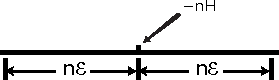
\includegraphics[width=0.35\textwidth]{images/range-ts.pdf}
  %\caption{.}
  \label{fig:range-ts}
  \end{figure}
\end{frame}


\begin{frame}%[allowframebreaks]
  \frametitle{Conjunto Típico}
  \begin{itemize}
  \item O tamanho do conjunto típico de sequências produzidas pela fonte é tipicamente
        muito menor que o tamanho do conjunto de todas as sequências produzidas pela fonte.
  \item Uma sequencia típica não precisa ter probabilidade próxima daquela que é a sequência mais provável.
  \item Geralmente a sequência mais provável não está no conjunto típico.
  \end{itemize}
\end{frame}


